\documentclass[a4paper,12pt]{article}
\usepackage[margin=1in]{geometry}
\usepackage[colorlinks = true, citecolor=red, urlcolor=blue]{hyperref}
\usepackage{listings}
\usepackage{graphicx}
\usepackage{subcaption}

\parindent=2pt
\parskip=1ex plus 0.5ex minus 0.2ex

\begin{document}

\title{Repeated games with mistakes}
\author{Nikolas M. Skoufis \\ Supervisor: Julian Garcia}
\date{October 20th, 2015}

\maketitle

\begin{abstract}

This project studies efficient methods to compute the expected payoff of an iterated prisoner's dilemma between two opponents.
In order to efficiently compute these payoffs, the mathematics underpinning the iterated prisoners dilemma and the computation of expected payoff was analyzed with a view to improving in speed of computation over existing methods.
A Monte-Carlo method of computing expected payoff was used as a benchmark against which two fast methods for computing payoff were compared.
The results of these fast methods were then used to generate three-population simplex plots of evolutionary dynamics as a further benchmark.

\end{abstract}

\section{Introduction}

\subsection{Prisoner's Dilemma}

The prisoner's dilemma is an archetypal problem in game theory, particularly in the study of the evolution of cooperation.
The prisoner's dilemma involves two prisoners, each of which has two moves available to them.
The prisoner's are told of the two options available to them, and they are told that they have 24 hours to make a decision or they will be punished.
Each player can either inform on the other player (known as \textit{defection}) or stay silent (known as \textit{cooperation}).
If both prisoners defect, will both spend 10 years in prison.
If both prisoners cooperate, they will each spend only 5 years in prison; a better outcome for both.
However if one prisoner cooperates and the other defects, the prisoner who defected goes free, and the prisoner that cooperated will spend 20 years in prison; longer than any other option.

Given these options and outcomes, we can see that a natural dilemma arises.
If a player cooperates, they may receive a better outcome than if they had defected, depending on the other player's action.
However if they defect, they have the opportunity for best possible outcome (going free), but they also risk punishment if the other player defects.
This problem is the prisoner's dilemma.

An important concept in game theory is that of the Nash equilibrium.
The Nash equilibrium is a set of strategies where each player cannot improve their own outcome by changing their strategy while the opponent's strategy remains the same.
This means that in effect, a Nash equilibrium is the optimal result for all players.
It is a well known result in game theory that the only Nash equilibrium in the prisoner's dilemma is for both players to defect.
However this result is only valid for the single-shot prisoner's dilemma ie. the prisoner's dilemma where the players only play the game once.
If players player multiple times, more complex strategies can emerge and there emerges an incentive for mutual cooperation~\cite{trivers}.
This problem is known as the `iterated prisoner's dilemma'.

One issue with the iterated prisoner's dilemma is that if players know ahead of time how many rounds of the prisoner's dilemma they will play, the cooperation breaks down.
Since there are no repercussions for defecting in the final round (because there are no more rounds in which the opponent can retaliate), it is always best to defect.
However if it is optimal for both players to defect in the final round, then logically there are no repercussions for defecting in the second-to-last round either.
By this logic, the optimal strategy is simply to always defect.
In order to overcome this predictable and uninteresting pattern, we introduce the idea that the game length is determined by a repeated random event.
After playing the first and subsequent rounds, the game continues for another round with probability $0 < \delta < 1$.
This means that there is a always a chance that there will be another round of the game, and thus there is always the possibility that defection will carry consequences.

\subsection{Expected Payoff}

The different moves and their respective outcomes of the prisoner's dilemma are generally abbreviated, and we will use these abbreviations from here onwards.
Cooperation and defection are usually abbreviated to C and D respectively.
The payoff for mutual cooperation is abbreviated to R for reward.
The payoff for mutual defection is abbreviated to P for punishment.
If one player defects and the other cooperates, the defector is said to receive the T (for temptation) payoff and the cooperator receives the S (for sucker) payoff.

When playing the iterated prisoner's dilemma, many different strategies are possible.
The most basic of strategies is to unconditionally perform the same action: unconditionally defect or unconditionally cooperate.
These strategies are known as Always Defect (AllD) and Always Cooperate (AllC) respectively.
More complicated strategies include:

\begin{itemize}
    \item Tit For Tat (TFT): If the opponent cooperate last round, you cooperate. If the opponent defected last round, you defect. In the first round, the player cooperates.
    \item Win Stay, Lose Shift (WSLS): If the outcome is a win for the player (R payoff or T payoff) then the previous move is repeated. If the outcome is a lose for the player (P payoff or S payoff) then the opposite move is chosen in the next round.
    \item Grim: Cooperates until the opponent defects, and then unconditionally defects from then on.
\end{itemize}

It is useful to be able to compare the effectiveness of each of these strategies when paired against another strategy.
For simple cases such as AllC against AllD, AllD is trivially the superior strategy.
However in more complicated cases, it becomes necessary to use a metric to evaluate the performance of a strategy.
The most commonly used metric is the expected payoff.

The expected payoff is defined as the expected value of the payoff of one strategy when pitted against another strategy.
For deterministic strategies, this can easily be computed with an infinite sum \cite{garciaandtraulsen}:

\begin{equation}
    \sum_{i=0}^{\infty} \delta^i \pi_i
\end{equation}

where $\delta$ is the continuation probability and $\pi_i$ is the payoff of the strategy in round $i$.

This sum holds for any pair of deterministic strategies.
This sum is straight-forward to compute programatically, however when we move to non-deterministic strategies it quickly becomes difficult.
Any strategy that employs non-deterministic play styles (eg. defect 75\% of the time, cooperate the other 25\%) introduces additional options in the outcome space which must be accounted for.
We must now multiply the continuation probability by the probability of that particular outcome, and we have to continue this `branch' of the outcome tree forever.
For more complex strategies, the space of outcomes quickly becomes very large, and consequently, the expected payoff becomes very difficult to compute.

\subsection{Mistakes and fault tolerant strategies}

Another possible complication of the outcome space is the addition of mistakes.
Mistakes occur when a player intends to play a particular move, but instead they play a different move.
In the context of the iterated prisoner's dilemma, this occurs when a player intends to cooperate, but instead they defect (or vice-versa).
Since mistakes are probabilistic and can occur at any round, they serve to worsen the problem of exploding outcome space and associated difficulty in calculating expected payoffs.
This project's primary goal was to determine a method of computing the expected payoff of an iterated prisoner's dilemma with mistakes in an efficient manner.

In the presence of mistakes, some strategies fare better than others.
In particular, it is a well known result \cite{axelrod} that the simple TFT strategy outperforms all other strategies in the absence of mistakes.
However in the presence of mistakes, the TFT strategy displays poor `fault tolerance' because it loses the `robustness' property.
For a rigorous definition of fault tolerance and robustness, refer to \cite{pelc} and \cite{pelcpelc}.
Briefly, robustness is a measure of how a strategy performs against another strategy in a population consisting only of those two strategies.
Informally, a robust strategy is said to be sometimes better and never worse than other strategies.
A fault tolerant strategy is a strategy that is able to retain this robust quality, even in the face of mistakes.

Since TFT is not particularly fault tolerant, modern game theorists have attempted to study strategies that are able to deal with faults while still remaining competitive.
And in order to evaluate these strategies, it becomes necessary to efficiently and easily calculate their expected payoffs against other strategies.

\section{Software tools and techniques}

In order to study the expected payoff, it was necessary to first design a software framework that allows for the construction, simulation and computation of scenarios in game theory.
The code used in this project is open sourced under the GNU GPL v3 license and is available at https://github.com/computationalevolutionarydynamics/repeatedmistakes.

Python was chosen as the language for development of this framework, due to both the author's familiarity with the language coupled with high quality libraries for numerical calculations, visualization and testing.
In particular, this project made use of the Hypothesis property-based testing library \cite{hypothesis} and the Nose testing framework \cite{nose}.
I also used the Travis CI continuous integration service and the Coveralls test coverage service.

\subsection{Hypothesis and Nose}
The Hypothesis library is inspired by the Haskell library `Quickcheck', and is a property-based form of testing.
The chief difference is that instead of defining in terms of specific inputs and outputs, you define tests in terms of classes of input and their expected output.
Hypothesis uses in intelligent search strategy to attempt to produce an input which falsifies the property.
Hypothesis then reduces this input to the minimum falsifying example and returns this.

As an example, here is how we might test a \texttt{reverse} method with conventional testing and with Hypothesis:

\begin{itemize}
    \item Conventional: when called with the input \texttt{foobar}, the method should return \texttt{raboof}.
    \item Hypothesis: when called with any string, the method should return the reverse of that string.
\end{itemize}

Clearly the Hypothesis version is much more powerful and expressive.
For example, if the \texttt{reverse} method didn't correctly handle empty strings, then Hypothesis would catch this and return it to the user.

Hypothesis proved to be an invaluable tool in this project because it allowed me to define the general properties that should be obeyed for any strategy and any history, and then evaluate my implementations of the strategies against these properties.

One issue I ran into with using Hypothesis was running tests can be slow when compared to standard unit testing.
For example, running a test to ensure that strategies always return the correct length of history over 8 different strategies can take on the order of seconds.
Although this is not a huge concern, this did cause some issues with Travis as discussed below.

Another issue with Hypothesis is that occasionally it would produce an error because it was unable to produce enough test data satisfied the requirements given.
This is most likely due to inexperience with Hypothesis, and could likely be remedied by optimizing the functions that construct test data.

Finally, since Hypothesis's testing is fundamentally probabilistic in nature, occasionally tests would fail even though the code that changed did not affect them.
This occurs because Hypothesis uses some randomized test data to find edge cases, and sometimes that test data doesn't hit upon a falsifying example.
This can be remedied by increasing the number of examples to test for each property, however there is always the possibility that a falsifying example will be skipped over.

In addition to Hypothesis, I made use of the Nose testing framework.
Nose aims to be a replacement for Python's default \texttt{unittest} library, with an emphasis on simpler and more readable test code.
A key reason behind my use of Nose is that Nose allows for what it calls `test generators'.
Test generators allow for generation of multiple tests over a variety of input data.
This feature was also useful when evaluating the correctness of the strategies that were implemented.

\subsection{Travis and Coveralls}

In order to easily keep track of the status of the unit tests, I used the Travis CI continuous integration service.
Travis CI can be configured to automatically build your project, and then to run any tests you have implemented.
Travis builds and runs the tests upon every Github commit, so it is a valuable tool in ensuring that new code does not cause tests to fail.

As mentioned in the previous section, some issues occurred when using Travis with Hypothesis.
Since some tests took a very long time to execute, an additional option had to be set in Travis to allow for long periods of time without output.
Even with this setting, builds sometimes failed because Travis has an upper limit on how long it will wait before timing out.

To assess the test coverage of the tests I had written, I used the Coveralls service.
This service integrates with Travis to automatically generate test coverage reports.

Both of these services offer badges (dynamically updated images) that can be displayed on Github so that it's easy to see at a glance whether your build is passing and how much of the code base is covered by your tests.

\section{Software framework}

In order to design and test alternate methods of computing expected payoff, we need a framework that supports creation and simulation of strategies and payoffs.
To this end I implemented a \texttt{Strategy} class which implements basic functionality of a strategy such as tracking the player's history and computing the next move for the player.
This \texttt{Strategy} class is never instantiated directly, but is instead subclassed by concrete implementations of strategies eg. \texttt{AllC}, \texttt{AllD}, \texttt{TitForTat} etc.
This implementation should allow for any strategy to be implemented (including non-deterministic strategies) since the method that computes the next move for the strategy knows about both the player's own history as well as being passed the opponent's history.

We also implement a class for defining a payoff structure known as a payoff matrix.
The payoff matrix encodes the payoffs for any combination of player actions, and so can be used to compute the payoff of a sequence of game results.

\section{Calculation strategies}

\subsection{Closed form solutions}

Closed form solutions for the expected payoff are known for combinations of simple strategies.
Results from \cite{garciaandtraulsen} were used to evaluate the simple strategies such as AllC, AllD, TFT and others that have the property that their behaviour is only dependent on at most the last move the opponent made.
These results were used to assess the accuracy of the different calculation methods during initial trials.

\subsection{Monte Carlo methods}

The most basic calculation strategy is to simply simulate a large number of random games and to average the results.
This class of methods are known as Monte Carlo methods.
These methods are relatively easy to implement, but because they are by their nature randomized, we must conduct a large number of trials in order to arrive at an accurate result.

One method of Monte Carlo simulation is to simply run a large, fixed number of trials.
Although this is easy to implement, it doesn't provide the user with any estimate of accuracy.
Accuracy of the result must simply be evaluated against known, closed form solutions where they are available.
Then the number of trials used can be assumed to be accurate for other situations for which a closed form solution is not available.

A more complex method of estimation is to compute the standard deviation of the estimator, and to stop conducting trials when this estimator standard deviation is within a certain threshold.
This method and its derivation is explain in \cite{ross}.
By computing the standard deviation of existing results, additional trials can be generated until eventually a guarantee of the accuracy of the answer is given.
This result gives you a guarantee that the difference between the true value and the estimate you have produced is distributed with a given standard deviation.

Both methods of Monte Carlo simulation where implemented, though in practice the former method was used because it is less computationally expensive and is also more widely used and understood.
Both methods were also reimplemented to make use of multiple processors using the Python \texttt{multiprocessing} library.
Since individual trials of the Monte Carlo simulation are independent, it is efficiently to compute the results of trials in parallel and to aggregate the results once trials have been completed.

\subsection{Brute force approach}

One approach to calculation is to simply compute all of the possible outcomes and their associated likelihoods, and to combine these as a weighted sum.
However as discussed above, in the presence of mistakes this quickly becomes prohibitively expensive.
At each round in a repeated game, there are four possible mistake related outcomes.
Both players can make no mistakes, either player can make a mistake, or both players can make a mistake.
Therefore, the number of possible paths via which a repeated game can evolve grows like $n^4$ where $n$ is the round number.

In order to attempt to control this explosion of outcomes, we can attempt to `prune' the outcome tree so that it is more manageable.
We can choose some cutoff term size $\epsilon$, so that when a particular term in the infinite sum (payoff multiplied by the probability of reaching that state) drops below the threshold $\epsilon$, we truncate that branch of the outcome tree.

In order to efficiently perform this calculation with pruning, we use a queue based algorithm.
After each term is computed, the associated history and the probability of reaching that state is stored on a queue, but only if the term that is produced is above the $\epsilon$ threshold.
This way, unlikely outcomes are pruned until all outcomes become sufficiently unlikely and the algorithm terminates.

The pseudocode for this algorithm can be found in listing \ref{calc_code}.

\lstinputlisting[language=python,float,label=calc_code,caption=An algorithm for efficiently estimating expected payoff,frame=tblr,breaklines=true]{calculation_pseudocode.py}

\subsection{Simplified approach}

Another approach to computing expected payoff is to take a greatly simplified approach which reduces the number of outcomes that must be explored.
This approach assumes that all games last a fixed length.
In order to achieve the most accurate result, this fixed game length is chosen to be the expected number of rounds given the continuation probability.
Since the length of games follows a geometric distribution, this value is $\frac{1}{\delta}$ where $\delta$ is the continuation probability.
With this added limitation we can use the similar algorithm to the one described in listing \ref{calc_code} but only for games of the given length.

\section{Results}

In order to evaluate the different methods for finding the expected payoff, all three methods were run over a range of inputs.
I tested all combinations of the following parameters:

\begin{itemize}
    \item Continuation probability: $0.5, 0.6, 0.7, 0.8, 0.9, 0.99, 0.999$
    \item Mistake probability: $0.1, 0.01, 0.0001, 0.00001, 0.000001$
\end{itemize}

For the calculation based methods, term cutoff sizes of 1e-4, 1e-5 and 1e-6 were were computed across all other combinations of parameters.
The calculation based code was executed on my personal computer.
For the Monte Carlo simulations, the simulations were run with 100,000 trials in the Monash Campus Cluster (see below).
Finally, each combination of strategies was run for each of the parameter combinations.
The strategies used were:

\begin{itemize}
    \item AllC
    \item Suspicious AllC
    \item AllD
    \item Nice AllD
    \item Tit For Tat
    \item Suspicious Tit For Tat
    \item Inverse Tit For Tat
    \item Suspicious Inverse Tit For Tat
    \item Win Stay, Lose Shift
    \item Grim
    \item Tit For 2 Tats
\end{itemize}

\subsection{Monash Campus Cluster}

The Monash Campus Cluster (MCC) was used to run the computationally intensive simulation code.
The MCC is a 200 server heterogeneous cluster, which means that it is composed of many machines with different hardware capabilities.
Some machines feature a high number of cores, some feature a low number of cores but a large amount of RAM, and others have GPU capabilities.

Submission of jobs to the cluster involves the use of the Sun Grid Engine job system.
Jobs are defined in .pbs files which contain information such as the maximum allowable resources for the job and the instructions to execute.
In order to speed up the process of making all of these job files and submitting them, I wrote a shell script
This scrip creates lots of job files and a single batch file to submit them all, based off of iterating through some arrays in which you can define the parameter values for the jobs.

Learning to execute code on the cluster proved to be a bit of a challenge.
In order to execute code on the cluster, all Python code had to be put into a single .py file.
In addition, the Python libraries installed on the MCC are limited, and installing additional libraries was not an option.
This presented some problems in data generation and analysis, because the output had to be collected in many small text files.
It would have been preferable to use a Python library such as \texttt{pandas} for the data collection, however this was not installed.

Multiprocessing on the cluster also proved difficult.
In order to enable multiprocessing, a special `parallel environment' option must be specified.
There are two such parallel environments on the MCC: the \texttt{smp} environment and the \texttt{orte\_adv} environment.
The \texttt{smp} environment executes the code on a single machine with the requested number of cores, while the \texttt{orte\_adv} environment executes your code across the requested number of cores, but potentially across multiple machines.
Since I wasn't sure that the code would work under the \texttt{orte\_adv} environment, I opted for the \texttt{smp} environment.
However this meant that some simulations did not execute in time for this report because the requested resources were being used by others on the cluster.

\subsection{Comparison of results}

Once all the results had been generated and collected from the cluster it was necessary to evaluate the calculation methods against the simulations.
For the purposes of this project, the simulation values were taken to be the `canonical' values, and the calculated values were compared against them.

Once of the chief advantages of the calculation methods were that they were fast.
The smart brute force method took on the order of seconds to execute
In contrast, the simulations took on the order of tens of minutes to execute on the powerful machines of the MCC.

Although the expected value only method was extremely fast (generally faster than a second), the results proved to be too inaccurate to be useful.
The only time when the expected value method may produce good results is when the continuation probability is small, because it concentrates all of the mass of the expected payoff near the expected value.
However the situations when the continuation probability is low is not often studied, and thus the usefulness of the expected value method is limited.

In terms of accuracy, as you might expect the calculations were more accurate for smaller minimum term sizes.
In general, the smart brute force method was accurate to within 1\% relative error for most combinations of continuation probability and mistake probability.
There was a general trend that relative error decreased for smaller mistake probability.
When the mistake probability is 0.1 or above, not only do the results for the smart brute force method rapidly degrade, but the calculation is also incredibly slow (on the order of 60 minutes in one particular case).
A table showing the relative error in expected payoffs fort Tit For 2 Tats against Inverse Tit For Tat can be seen in figure \ref{error_table}.

\begin{figure}
    \caption{A table of the relative error in expected payoffs for the strategy Tit For 2 Tats against the strategy Inverse Tit For Tat in the iterated prisoner's dilemma. Parameters: term cutoff size: 1e-6, number of Monte Carlo trials: 100,000}
    \label{error_table}
    \centering
        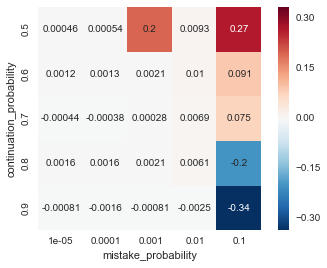
\includegraphics[width=0.5\textwidth]{error_table}
\end{figure}

Since the eventual goal of this research is to use the expected payoff as part of computational evolutionary dynamics simulations, it seemed prudent to run a few of these simulations with the results we obtained.
The purpose and derivation of the figures found in figures \ref{simplex_good} and \ref{simplex_bad} are beyond the scope of this report.
However in brief, these plots show how a populations consisting of individuals that play one of three strategies evolves according to `replicator' dynamics.
In these plots, the expected payoffs are used to determine the relative `fitness' of the strategies, and this fitness determines how often each strategy reproduces.
In figures \ref{simplex_good} and \ref{simplex_bad}, the states where the population is entirely composed of players of one strategy are in the corners.
The arrows in the figures represent the direction of movement of the population distribution, and the coloration represents the speed at which the populations moves in these directions.

\begin{figure}
    \caption{Simplex plots of the interaction between AllC, AllD and Tit For Tat. Parameters are continuation probability = 0.9, mistake probability = 0.0001. For the calculations the term cutoff size is 1e-6 and the number of Monte Carlo trials for the simulations is 100,000}
    \label{simplex_good}
    \centering
        \begin{subfigure}[b]{0.5\textwidth}
            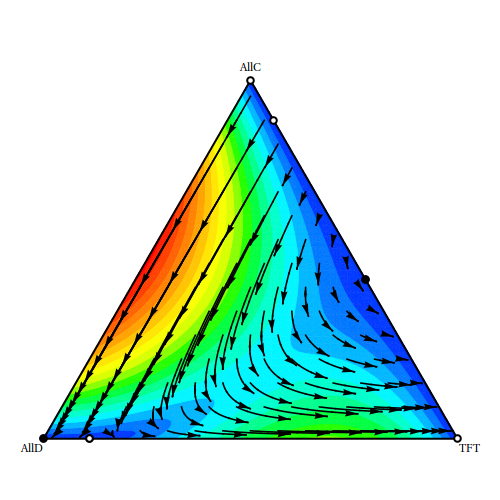
\includegraphics[width=\textwidth]{simplex_good_calcs}
            \caption{Calculations}
        \end{subfigure}
        \begin{subfigure}[b]{0.5\textwidth}
            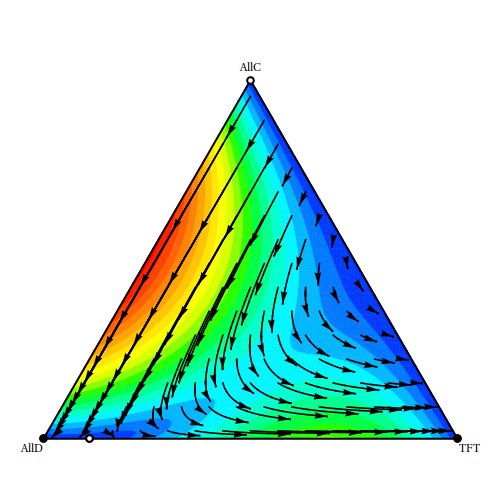
\includegraphics[width=\textwidth]{simplex_good_sims}
            \caption{Simulations}
        \end{subfigure}
\end{figure}

\begin{figure}
    \caption{Simplex plots of the interaction between Tit For Tat, Tit For 2 Tats and Win Stay, Lose Shift. Parameters are continuation probability = 0.9, mistake probability = 0.0001. For the calculations the term cutoff size is 1e-6 and the number of Monte Carlo trials for the simulations is 100,000}
    \label{simplex_bad}
    \centering
        \begin{subfigure}[b]{0.5\textwidth}
            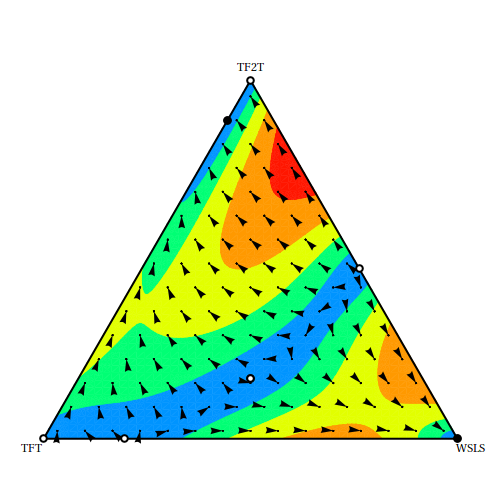
\includegraphics[width=\textwidth]{simplex_bad_calcs}
            \caption{Calculations}
        \end{subfigure}
        \begin{subfigure}[b]{0.5\textwidth}
            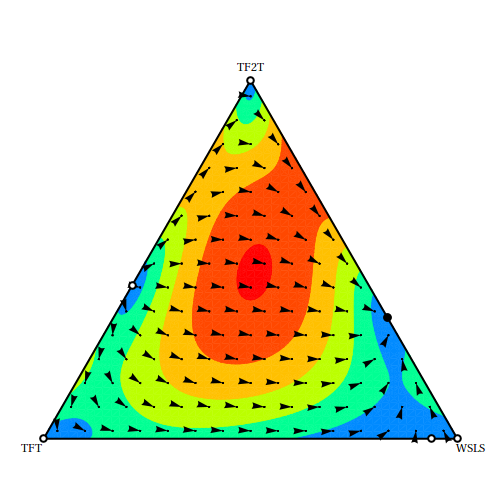
\includegraphics[width=\textwidth]{simplex_bad_sims}
            \caption{Simulations}
        \end{subfigure}

\end{figure}

As you can see, figure \ref{simplex_good} shows results where the calculations and simulations produce very similar phase plots.
However in figure \ref{simplex_bad} shows results where the calculations and simulations produce very different phase plots.
Despite the fact that the relative error is roughly the same in both of these cases, my theory is that the sensitivity of the results to the initial expected payoffs causes this stark difference.
This may indicate that the expected payoff method is only useful for certain combinations of strategies.
Alternatively, since the simulations are prone to some error as well, it may simply indicate that this combination of strategies is very chaotic and is highly dependent on individual mistakes at key moments.

\section{Conclusion and future directions}

In this project I have explored alternate methods of calculating the expected payoff of different strategies playing the iterated prisoner's dilemma with mistakes.
I have designed and implemented a software framework for studying the iterated prisoner's dilemma, as well as methods for simulating and calculating expected payoffs.
I have also gained valuable skills using Travis, Coveralls, Nose and Hypothesis for continuous integration and testing.
The results from the data I have produced seem to indicate that the brute force method is accurate across a wide variety of parameters and strategies, as long as the mistake probability is less than 0.1.
Unfortunately, the expected value method doesn't produce satisfactory results.

Due to time constraints, I could not complete as thorough an analysis of the data that was produced as I would have liked.
Additional analysis of the data could be undertaken, with the aim of identifying trends in the accuracy of results.
It may be that certain strategies produce more accurate results than others.

In addition, further examination of simplex plots and results produced by evolutionary dynamics calculations may reveal additional patterns.
Preliminary analysis seems to indicate that when all of the expected payoffs are close together, even the small differences between the simulations and the calculations can produce vastly different results.
Since this is the intended usage of these methods, further analysis of the actual results of simulations would be a good indicator towards the viability of the calculation methods.

\begin{thebibliography}{9}

    \bibitem{axelrod}
        Robert Axelrod,
        \emph{Effective choice in the Prisoner's Dilemma},
        The Journal of Conflict Resolution,
        Vol. 24,
        No. 1,
        1980.

    \bibitem{pelcpelc}
        Andrzej Pelc, Krzysztof J. Pelc,
        \emph{Same Game, New Tricks: What Makes a Good Strategy in the Prisoner's Dilemma?},
        The Journal of Conflict Resolution,
        Vol. 35,
        No 5,
        2009.

    \bibitem{pelc}
        Andrzej Pelc,
        \emph{Fault-tolerant strategies in the Iterated Prisoner's Dilemma},
        Information Processing Letters,
        Vol. 110,
        No. 10,
        2010.

    \bibitem{garciaandtraulsen}
        Julian Garcia, Arne Traulsen,
        \emph{The Structure of Mutations and the Evolution of Cooperation},
        PLoS ONE,
        Vol. 7,
        No. 4,
        2012.

    \bibitem{trivers}
        Robert Trivers,
        \emph{The Evolution of Reciprocal Altruism},
        The Quarterly Review of Biology,
        Vol. 46,
        No. 1,
        1971.

    \bibitem{hypothesis}
        David R. MacIver,
        \emph{Hypothesis},
        https://github.com/DRMacIver/hypothesis,
        2015.

    \bibitem{nose}
        \emph{Nose},
        https://nose.readthedocs.org/en/latest/index.html,
        Version 1.3.7.

    \bibitem{ross}
        Sheldon M. Ross,
        \emph{Simulation},
        Fourth edition,
        Elsevier Academic Press,
        2006.

\end{thebibliography}

\end{document}
